\documentclass[runningheads]{llncs}
	\usepackage[ngerman,english]{babel}  % Language specification
	\usepackage{varioref}  % Better references but possibly unstable
	\usepackage[T1]{fontenc}  % Output umlauts in a PDF
	\usepackage[utf8]{inputenc}
	\usepackage{pslatex}
	\usepackage{amsmath}
	\usepackage{multirow}
	\usepackage{ellipsis}
	\usepackage{textcomp}
	\usepackage{longtable}
	\usepackage{rotating}
	\usepackage[section]{placeins}

	\usepackage[inline]{enumitem}  % Inline enumeration capability
	\usepackage[font=small,labelfont=bf]{caption}  % Customize caption aesthetics
	\usepackage[font=small]{subcaption}  % Customize sub-captions

	\usepackage{color}
	\usepackage{xcolor}  % Highlighting
	\usepackage{tcolorbox}  % Fancy colored boxes
	\usepackage{soul}

	\usepackage[tracking=true]{microtype}  % Change character spacing

	\usepackage{graphicx}  % Insert images
	\usepackage{listings}  % Insert programming code
	\usepackage[space]{grffile}  % Insert images baring a filename which contains spaces
	\usepackage{float}  % Forcefully set the location of an object

	\usepackage[style=numeric,sorting=none,backend=biber]{biblatex}  % Reference manager
	\usepackage[bookmarks]{hyperref}  % Clickable references

	\usepackage[nodayofweek]{datetime}  % Flexible date specification
	\usepackage{scrextend}  % Arbitrary indentation

	\addbibresource{../literature.bib}

	% Display URLs in blue roman font if using hyperref to comply with Springer's eBook style
	\renewcommand\UrlFont{\color{blue}\rmfamily}

	\makeatletter
	% Insert a float barrier before subsections just like the package 'placeins' does for sections
	%\AtBeginDocument{%
	%	\expandafter\renewcommand\expandafter\subsection\expandafter{%
	%		\expandafter\@fb@secFB\subsection
	%	}%
	%}
	\makeatother
	\setlength{\intextsep}{1em}  % Reduce excessive spacing between float and text
	%\setlength{\textfloatsep}{1em}  % Reduce excessive spacing between caption and text

	% Use bold sub-caption references
	\DeclareCaptionLabelFormat{bold}{\textbf{#2}}
	\captionsetup{subrefformat=bold}

	\pagenumbering{gobble}  % Disable page-numbering

	%\parindent0em  % Indentation of the first line of a paragraph
	\newcommand{\leadingzero}[1]{\ifnum#1<10 0\the#1\else\the#1\fi}
	\newcommand{\todayddmmyyyy}{\leadingzero{\day}.\leadingzero{\month}.\the\year}
	\newcommand{\mathcolorbox}[2]{\colorbox{#1}{$\displaystyle #2$}}
	\renewcommand{\sectionautorefname}{\ifnum\spacefactor>1000 Section\else section\fi}  % Capitalize 'section' if used after some spacing
	\def\permille{\ensuremath{{}^\text{o}\mkern-5mu/\mkern-3mu_\text{oo}}}  % Permille sign

	\lstset{basicstyle=\ttfamily,breaklines=true}  % Prettier code highlighting style
	\pagestyle{empty}  % Prettier page format without header and footer

\begin{document}

\titlerunning{Augmenting the DonorsChoose.org Corpus for Meta-Learning}  % Abbreviated title
\title{Augmenting the DonorsChoose.org Corpus for Meta-Learning%
	\thanks{This publication emanated from research conducted with the financial support of Science Foundation Ireland (SFI) under Grant Number 13/RC/2106.}}
\author{Gordian~Edenhofer\inst{1,2} \and Andrew~Collins\inst{1} \and Akiko~Aizawa\inst{2} \and Joeran~Beel\inst{1,2}}
\authorrunning{G. Edenhofer et al.}  % Abbreviated author field
\institute{
	Trinity College Dublin, School of Computer Science \& Statistics, ADAPT Centre, Ireland\\ \and
	National Institute of Informatics Tokyo, Digital Content and Media Sciences Division, Japan\\ \email{beelj@tcd.ie, collinsa@tcd.ie, aizawa@nii.ac.jp}
}

\maketitle  % Typeset the header of the contribution
%\markboth{}{}  % Clear the section and author from the page header; also see `\pagestyle`

\begin{abstract}
The DonorsChoose.org dataset of past donations provides a big and feature-rich corpus of users and items. The dataset matches donors to projects in which they might be interested in and hence is intrinsically about recommendations. Due to the availability of detailed item-, user- and transaction-features, this corpus represents a suitable candidate for meta-learning approaches to be tested. This study aims at providing an augmented corpus for further recommender systems studies to test and evaluate meta-learning approaches. In the augmentation, metadata of collaborative and content-based filtering techniques is amended to the corpus. It is further extended with aggregated statistics of users and transactions and an exemplary meta-learning experiment. The performance in the learning subsystem is measured via the recall of recommended items in a Top-N test set. The augmented dataset and the source code are released into the public domain at \href{https://github.com/BeelGroup/Augmented-DonorsChoose.org-Dataset}{GitHub:BeelGroup/Augmented-DonorsChoose.org-Dataset}.

\keywords{recommender systems \and meta-learning \and dataset augmentation \and ensemble learning \and hybrid recommenders.}
\end{abstract}

\section{Introduction}
Meta-Learning is the process of applying machine learning algorithms on metadata of previous machine learning experiments. The goal is to improve existing approaches by combining the strengths of several single machine learning systems~\cite{AIR:MetalearningSurveyOfTrendsAndTechnologiesLemke2015}. In recommender systems it is an emerging field of interest as meta-learning promises to utilize patterns in metadata as to retrieve the best possible match of item and user. In order to investigate meta-learning algorithms, the required metadata needs to be computed in advance.

One challenge for researchers interested in meta-learning is that suitable datasets are time-consuming and cumbersome to construct. Creating a system of individual machine learning experiments and amending their metadata to the original corpus takes time and resources away from working with the actual meta-learners. Multiple examples of manual and repetitious data augmentation may be found in the scientific literature, for instance in~\cite{CUNHA2018128,DBLP:journals/corr/abs-1805-12118,Ekstrand:2012:RFP:2365952.2366002}. Furthermore, the choice of the metric for computing metadata of single machine learners is important. Using the RMSE, as is done in some of the aforementioned publications, disallows using content-based methods.

Our objective is to address the data augmentation part in a comprehensive and reproducible~\cite{UMUAI:TowardsReproducibilityInRecSysBeel2016} way as to allow researchers to focus on the actual meta-learning task. We are presenting a public domain dataset which to our best knowledge has not been used for meta-learning before in the scientific community, yet due to its feature-rich and vast corpus is a suitable candidate. The raw dataset is augmented with metadata of several machine learning algorithms from a variety of fields (cf.~\cite{DBLP:journals/corr/abs-1805-12118}). In place of a metric, the recall in a Top-N set is used as it can be computed for a wide range of algorithms. The dataset is further amended with aggregated statistics about users and items, and metadata of an exemplary experiment.

\section{Methodology}

\subsection{The Dataset}
DonorsChoose.org is an organization which enables teachers to file project requests for resources for their school. Collectively the nonprofit has raised $\$685$ million for classrooms in the United States of America. Their dataset composed of past donations features $4.69$ million transactions performed by $2.12$ million users having donated to $1.11$ million projects. The corpus provides significantly more transactions with more detailed item and transaction information compared to, e.g., the popular MovieLens dataset. An exemplary itemized view of the augmented dataset is shown in~\autoref{tab:IllustrativeTable}.

The corpus features comprehensive information on the users (donors), items (projects) and transactions respectively interactions (donations). Transactions are represented by an interaction of a user with an item at a specific point in time and further include a strength (amount~donated). Users feature information about their location and a boolean value indicating whether they are a teacher. Items feature multiple textual descriptions, funding goals, a list of associated categories and types, information about the creator and details about the location of the school which the item is about.

In a first step, two collaborative filtering techniques and two content-based filtering techniques are applied. The performance measures of the single algorithms are amended to the table. Next, aggregated user and item statistics are calculated and added to the table. Lastly, four exemplary meta-learners are applied and the performance measures of the individual approaches are added to the corpus.

\begin{table}[ht]
	\centering
	\caption{Illustrative example of the overall design of the augmented transaction table with amended learning subsystem performance scores, statistics and meta-learner information.}%
	\label{tab:IllustrativeTable}
	\includegraphics[width=\textwidth,height=0.5\textheight,keepaspectratio]{{{../res/table}}}
\end{table}

\subsection{Dataset Preparation}
To prepare the dataset for evaluations, duplicate interactions are merged as the recommender systems shall not recommend items to which the user has already donated to. Internal stop words in description strings of items are stripped. Furthermore, transactions containing no information about the user's location are dropped thereby enabling the consistent usage of a user's location information in new approaches.

Additionally, users having interacted less than twice are removed as well. Although, this limits the target group, the step is unavoidable as the employed validation process requires at least one interaction per user for testing and one for training. The evaluation requires user profiles and hence training-transactions in order to recommend new items which in turn need to be validated against test-transactions. Lastly, the donated amount is transformed to a transaction strength in the range of unity to five in analogy to a rating score. This step reduces the influence of outliers respectively uncommon donated amounts.

\subsection{Learning Subsystem}
The learning subsystem is a recommender system itself. SVD and KNN are used as representatives for collaborative filtering techniques and TF-IDF and word-embedding as content-based filters~\cite{scikit-learn,rehurek_lrec}. Hereby, the otherwise intrinsic inductive bias is reduced. The word-embedding relies on fastText and utilizes pre-trained vectors~\cite{DBLP:journals/corr/BojanowskiGJM16}. Vector representations of items are the normalized sum of the vectors of the normalized embeddings of the individual words. In order to work with the data in an efficient way, transactions are sampled. For this study a sample-size of $100,000$ was chosen. This represents a fair balance between required computing time and ability to generalize.

The recall in a Top-N test set is used as score of how good an algorithm is able to recommend an item.
\begin{enumerate*}[label= (\arabic*)]
	\item For each user, first $100$ items with which the user has not interacted with are selected.
	\item The algorithm is then requested to rank an item with which the user has interacted with but which was not used for building the user's profile and the $100$ randomly sampled items. It is assumed that the random $100$ items are of low interest to the user.
	\item The position of the item with which the user has interacted with in the ranked test set may now be taken as the recall in a Top-N test set.
\end{enumerate*}

A classical 5-fold cross-validation on the users is applied for training the collaborative filters. An ordering is assumed to be implied by the magnitudes of the values in the reconstructed matrix of the decomposition respectively the distances to the neighbors. The validation process of the content-based approaches uses leave-one-out. The ranking is performed using the cosine similarity of an item's vector and the user's profile.

The choice of evaluation method ensures that it can be applied to a vast set of different algorithms as long as a ranking of items can be produced. Therefore, it allows for a high variety within the set of algorithms in the learning subsystem in contrast to, e.g., RMSE. It further ensures that not just the ability to decompose the data is measured but the ability to recommend new items to users~\cite{Cremonesi:2010:PRA:1864708.1864721}. Hereby, the learning subsystem is kept extensible while still providing useful metadata to meta-learning algorithms.

\subsection{Statistics and Application of Learning Subsystem}
The meta-learning system processes the metadata of the learning subsystem and further statistics. Its performance is evaluated via a holdout split on the transaction table using $80\%$ for training and the rest for testing. Transactions are expanded to contain more detailed information about the time, the user's location and aggregated statistics about the mean of the categories, location and interaction-strength of items with which the user has interacted with. Statistics are solely based on the training set. Values for unknown users are filled with the mean in the training data.

Four different meta-learning approaches are discussed which address the Algorithm Selection Problem (\textbf{ASP}) via a switching hybrid ensemble. The aim of the system is to predict the algorithm with the lowest recall-position for each transaction respectively each row in~\autoref{tab:IllustrativeTable}. The overall performance of a meta-learner is measured using the mean recall-position for when the recommended algorithm for each transaction is used.

The first approach aims at predicting the algorithm which will best describe the transaction via a classification based on the given meta-features using a decision tree. The second approach employs a gradient boosting regressor to predict the position of the recall for each transaction and for each algorithm in the learning subsystem separately. As best algorithm, the one with the lowest predicted recall-position is chosen.

The third meta-learner is a classical stacking ensemble using a decision tree which is given the prediction from the learning subsystem as additional input. Based on that, it performs a transaction classification. The final approach aims at solving the ASP via clustering transactions based on the meta-features using K-Means and assigns clusters an overall best algorithm via majority voting.

\section{Results}
The preparation of the dataset preserves a little more than half of the data with the most notable drop in the number of transactions being introduced by requiring users to have donated at least twice. The sample of $100,000$ transactions contains $18,735$ unique users and $88,100$ unique projects.

\begin{figure}[ht]
	\centering
	\subcaptionbox{Interaction Frequency\label{fig:InteractionFrequency}}{
		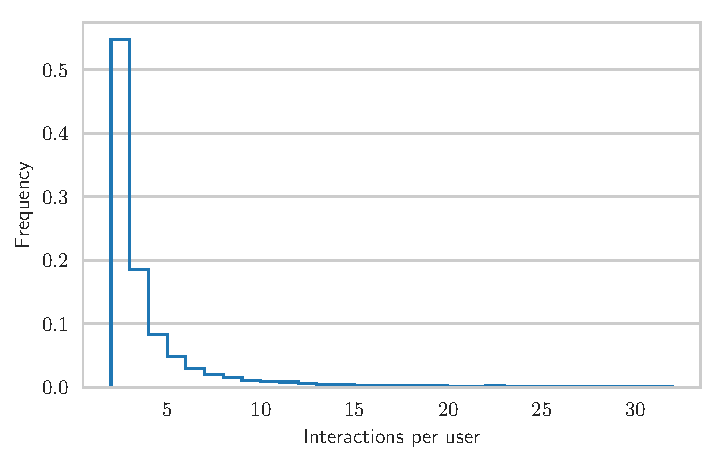
\includegraphics[width=0.45\textwidth,height=\textheight,keepaspectratio]{{{../res/number_interactions}}}
	}
	\hspace{2em}
	\subcaptionbox{Interaction Strength\label{fig:InteractionStrength}}{
		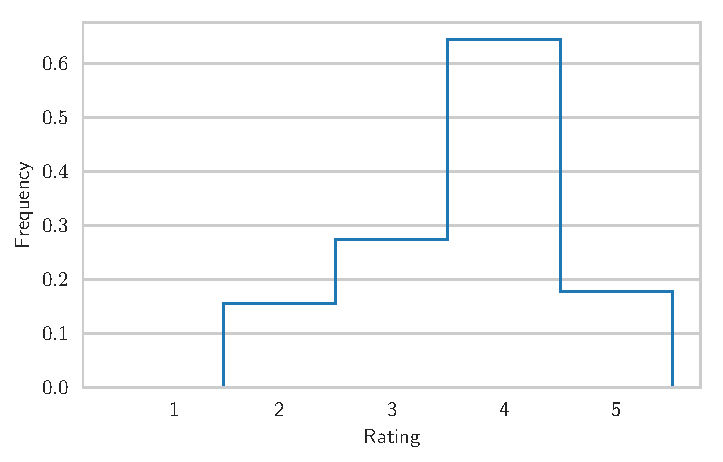
\includegraphics[width=0.45\textwidth,height=\textheight,keepaspectratio]{{{../res/distribtion_ratings}}}
	}
	\caption{The frequency of the number of interactions per user without outliers is shown in~\subref{fig:InteractionFrequency} and the distribution of the transformed interaction strength is shown in~\subref{fig:InteractionStrength}.}\label{fig:Interactions}
\end{figure}

Requiring users to have interacted at least twice, results in a distribution of the number of interactions per user which decays exponentially as depicted in~\autoref{fig:InteractionFrequency}. This is to be expected as the time and interaction strength (budget) a user can invest is limited. The dataset is dominated by users which interacted exactly two times.

The distribution of the transformed interaction strength in analogy to a rating score is shown in~\autoref{fig:InteractionStrength}. It peaks at the second highest score. Interactions with a weak to medium interaction strength and ones with the strongest interaction strength are about equally likely. Interactions with the lowest strength value are very infrequent.

\begin{figure}[ht]
	\centering
	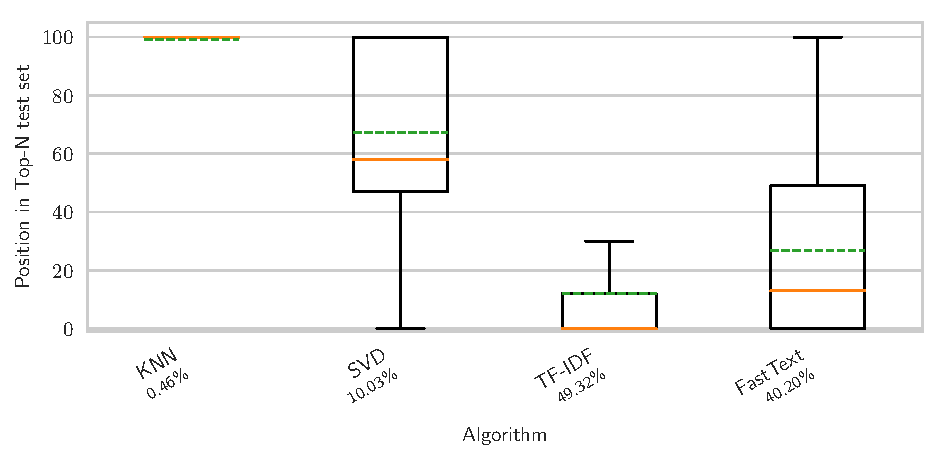
\includegraphics[width=\textwidth,height=0.3\textheight,keepaspectratio]{{{../res/learning_subsystem_position}}}
	\caption{Statistical features of the distributions of the recall-positions of the learning subsystem. The dashed green lines indicate the mean, the straight orange lines the median. The percentage below each algorithm indicates how often it is the best possible algorithm. To resolve a draw deterministically, the ``best'' algorithm is decided in alphabetic order.}%
	\label{fig:MetaLearnerStatistics}
\end{figure}

Statistical information about the performances are visualized in~\autoref{fig:MetaLearnerStatistics}. It can be observed that the performance of the learning subsystem depends highly on the employed filtering techniques. Overall, content-based filters are significantly better in achieving a low recall-position (average position in Top-N set; content-based filtering:~$19.48$, collaborative filtering:~$83.28$). The algorithm with the poorest performance is KNN. SVD performs better but is still unable to reliably yield good recommendations. Grouping users by shared item interactions has no observable positive impact on the recommendation.

Considering the low average number of interactions per user and the vast number of items available, KNN apparently fails to find appropriate neighbors. SVD seems to struggle with the sparsity of the input matrix as looking at the reconstruction of the decomposed matrix it is revealed that most values are well below unity and very similar to each other. SVD yields recall-positions below $10$ infrequently.

Content-based filtering techniques achieve better performance scores on the dataset. User profiles based on TF-IDF and fastText each yield recall-positions below $10$ for roughly half of all transactions with the simpler TF-IDF performing slightly better than fastText. This could be at least in part due to users explicitly searching for specific terms instead of exploring all possible items manually.

Between the different meta-learning approaches, significant changes in the mean recall-position can be noted as seen in~\autoref{fig:MetaLearnerPerformance}. The worst performer is the user-clustering using K-Means (average position in Top-N:~$15.56$). The stacking decision tree performs best (average position in Top-N:~$9.02$). Of the three non-stacking approaches the gradient booster performs best (average position in Top-N:~$11.21$) and achieves a better score than the single best algorithm, i.e., TF-IDF (average position in Top-N:~$11.96$). The classifying decision tree (average position in Top-N:~$15.27$) outperforms the user-clustering but is still notably worse than the overall best algorithm.

\begin{figure}[ht]
	\centering
	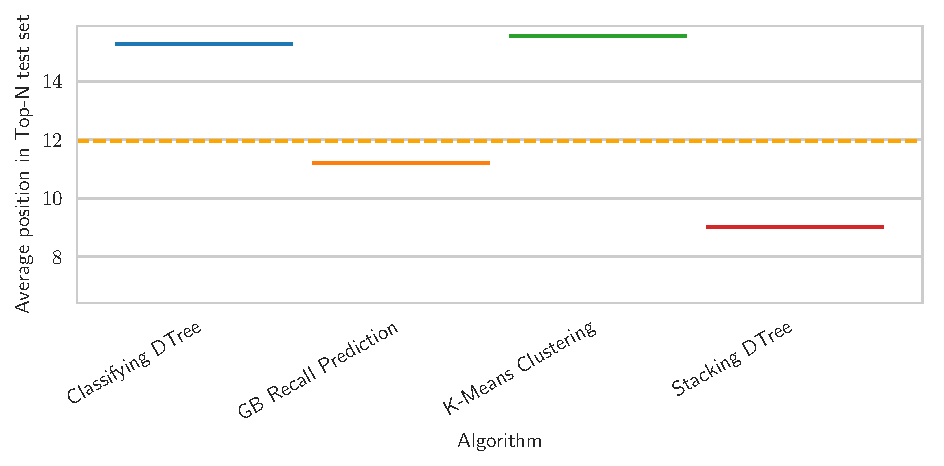
\includegraphics[width=\textwidth,height=0.3\textheight,keepaspectratio]{{{../res/meta_learner_performance_average_position}}}
	\caption{Performance of the meta-learner system addressing the ASP. The dashed orange line represents the overall best algorithm, i.e., TF-IDF.}%
	\label{fig:MetaLearnerPerformance}
\end{figure}

The fact that the stacking ensemble performs best is unsurprising as it is provided significantly more information than the other algorithms. The performance of the gradient booster is encouraging as it successfully addresses the ASP. From the poor performance of the user-clustering it can be reasoned that similar transactions do not necessarily yield similar results using the same recommender algorithm. Hence, the similarity of meta-feature does not imply that the performance of recommendations is similar.

The classification and error prediction approach apparently suffer from the level of indirection which is introduced by predicting a single algorithm and disregarding the penalty which is introduced if a bad performing one is chosen. Even a high accuracy in algorithm selection does not guarantee a low mean recall-position. This is partly mitigated by the error prediction approach but still not completely suppressed.

\section{Conclusion}
The study provides an extensively augmented dataset based on the transaction data published by DonorsChoose.org. The corpus is amended with metadata of individual recommender algorithms. Collaborative and content-based filtering techniques are used in the process and their performance is evaluated via the recall in a Top-N test set. Aggregated user and item statistics are amended to the table. Furthermore, Metadata of four switching hybrid ensemble meta-learners is amended to the dataset. The augmented public domain dataset lays the groundwork that future evaluations of existing and novel meta-learning approaches can build upon.

\begin{appendix}
	\printbibliography[heading=bibintoc]
\end{appendix}

\end{document}
